\documentclass[%
hyperref={colorlinks, citecolor=blue},
]{beamer}
\usepackage{unicode-math}
\usepackage{pgfplots}
\usepackage{listings}
\usepackage{qrcode}

% The code below is adapted from the style given in the following Overleaf article:
% https://www.overleaf.com/learn/latex/Code_listing
% Colors for syntax highlighting
\definecolor{codegreen}{rgb}{0,0.6,0}
\definecolor{codegray}{rgb}{0.5,0.5,0.5}
\definecolor{codepurple}{rgb}{0.58,0,0.82}
\definecolor{backcolour}{rgb}{0.95,0.95,0.92}

\lstdefinestyle{pythonstyle}{
  backgroundcolor=\color{backcolour},
  commentstyle=\color{codegreen},
  keywordstyle=\color{magenta},
  numberstyle=\tiny\color{codegray},
  stringstyle=\color{codepurple},
  basicstyle=\ttfamily\footnotesize,
  breakatwhitespace=false,
  breaklines=true,
  captionpos=b,
  keepspaces=true,
  numbers=left,
  numbersep=5pt,
  showspaces=false,
  showstringspaces=false,
  showtabs=false,
  tabsize=2
}
\lstset{%
  language=python,
  numbers=left,
  style=pythonstyle,
}

\newfontfamily\Raleway[Ligatures=TeX]{Raleway}
\newfontfamily\Lato[Ligatures=TeX]{Lato}

\usefonttheme{professionalfonts}

\setsansfont{Lato}[
UprightFont=*-Regular,
ItalicFont=*-Italic,
BoldFont=*-Medium,
BoldItalicFont=*-MediumItalic
]

\setmathfont{Lete Sans Math}[
CharacterVariant={3, 6}, % varepsilon/varphi defaults
]

\setbeamercovered{transparent}
% \setbeameroption{show notes on second screen=right}

\setbeamerfont{headline}{family=\Raleway}
\setbeamerfont{headline title}{size=\Huge,series=\bfseries}
\setbeamerfont{headline author}{size=\Large}
\setbeamerfont{headline institute}{size=\normalsize}
\setbeamerfont{block title}{family=\Raleway,size=\large,series=\bfseries}
\setbeamerfont{heading}{family=\Lato,series=\bfseries}
\setbeamerfont{caption}{size=\small}
\setbeamerfont{footline}{family=\Raleway,size=\normalsize}

\usetheme{moloch}

\definecolor{wvwcorange}{HTML}{F05123}
\definecolor{wvwcgray}{HTML}{949CA1}
\definecolor{lightorange}{RGB}{255, 240, 230}
\definecolor{lightgray}{RGB}{240, 240, 240}

\molochset{%
  progressbar=foot,
  block=fill,
}

\molochcolors{%
  title separator=wvwcorange,
  progressbar bg=wvwcgray,
  progressbar fg=wvwcorange,
  frametitle bg=wvwcorange,
  standout bg=wvwcorange,
}

% Alert Block
\setbeamercolor{block title alerted}{fg=wvwcorange,bg=lightorange}
\setbeamercolor{block separator alerted}{bg=black}
\setbeamercolor{block body alerted}{fg=black,bg=lightorange}

% Example Block
\setbeamercolor{block title example}{fg=wvwcorange,bg=lightorange}
\setbeamercolor{block separator example}{bg=black}
\setbeamercolor{block body example}{fg=black,bg=lightorange}

% Itemize
\setbeamercolor{item}{fg=wvwcorange}

\NewDocumentCommand{\rlang}{}{\textsf{R}}
\NewDocumentCommand{\pythonlang}{}{\textsf{Python}}

\usepackage[%
citestyle=numeric,
sorting=none,
natbib,
]{biblatex}
\addbibresource{local-bib.bib}

\title{Free and Open Source Tools for Research}
\author[J. Oldroyd]{Jesse Oldroyd}
\date[2026/06/15]{June 15, 2026}
\titlegraphic{\hfill
\includegraphics[width=3.5cm]{W_mountain-eps-converted-to.pdf}}

\begin{document}
\maketitle

\section{What is FOSS?}

\begin{frame}[<+->]
    \frametitle{Definition}
    \textbf{Free and open source software} (FOSS) is software
    \begin{itemize}
        \item that is freely available (usually under a permissive license);
              \vfill
        \item has accessible source code.
              \vfill
    \end{itemize}

    \begin{alertblock}{Free vs.\ Open}
        More restrictive definitions exist \cite{OpenSourceGNU2007}!
        \note[item]{Some define free software as the antithesis of proprietary software, whereas open software is treated more permissively.}
    \end{alertblock}
    \vfill
\end{frame}

\begin{frame}
    \frametitle{Philosophy of Free Software}
    The philosophy of free software can be encapsulated by \textit{four essential freedoms}~\cite{PhilosophyGNUProject}:
    \begin{enumerate}
        \item<2-> to use the software.
              \vfill
        \item<3-> to inspect and change the software.
              \vfill
        \item<4-> to share copies of the original software.
              \vfill
        \item<5-> to share copies of the modified software.
              \vfill
    \end{enumerate}
\end{frame}

\begin{frame}[<+->]
    \frametitle{Licenses}
    The freedoms associated with the use of free software are given legal weight by various \alert{licenses}, classified as \textit{copyleft} or \textit{permissive}~\cite{ChooseLicenseOpen}.
    \begin{itemize}
        \item Copyleft licenses: protects against proprietary software development.
              \note[item]{ Copyleft licenses can be used if you're planning to use your software for commercial purposes.}

              \vfill

        \item Permissive: encourages adoption and collaboration.
              \note[item]{Permissive licenses allow for your work to be used in commercial contexts.}

              \vfill
    \end{itemize}

\end{frame}

\begin{frame}[<+->]
    \frametitle{When FOSS Is the Right Choice}
    FOSS might be the right choice if you require
    \begin{itemize}
        \item Transparency.
              \note[item]{%
                      Transparency lets you inspect software itself to verify results.
                      Code that uses proprietary software makes it difficult, if not impossible, to confirm the correctness of results or to identify errors.
                  }

              \vfill
        \item Composability.
              \note[item]{%
                      Free software is often text-based.
                      Since so many use this common format, it can be relatively painless to chain multiple tools together into a single workflow.
                  }

              \vfill

        \item Customizability.
              \note[item]{%
                      Given how permissive many open source tools are, it's possible (and often expected) for you to customize the tool to your own needs.
                  }

              \vfill
    \end{itemize}
\end{frame}

\begin{frame}[<+->]
    \frametitle{When FOSS Is the Wrong Choice}
    Despite good reasons to use them, free and open source tools are not always a good idea.
    You need to be mindful of the following:
    \begin{itemize}
        \item Use tools that work well with what your collaborators are using.
              \note[item]{
                      In particular, follow any relevant journal guidelines!
                  }

              \vfill

        \item FOSS tools are often not as polished as their proprietary counterparts.
              \note[item]{
                      FOSS tools are also more subject to becoming ``abandonware'' as maintaining them is time-consuming—and often thankless—work.
                  }

              \vfill

        \item Security concerns.
              \note[item]{%
                      While many open-source projects are well-maintained, their accessibility to the public does leave them at risk of being used by malicious actors.
                      You should only use tools from trustworthy sources!
                  }

              \vfill
    \end{itemize}
\end{frame}

\section[Tools]{FOSS Tools}

\begin{frame}[<+->]
    \frametitle{Types of Tools}
    \begin{itemize}
        \item There is a large selection of open source tools available, including \alert{coding} and \alert{writing}.

              \vfill

        \item One of the most fundamental tools is a text editor.

              \vfill

        \item Even though you start with text, output is not
              necessarily just a text file!

              \vfill
    \end{itemize}
\end{frame}

\subsection{Coding}

\begin{frame}[<+->]
    \frametitle{Tools for Computation}
    \begin{itemize}
        \item \rlang

              \vfill

        \item \pythonlang\ with pandas, Seaborn and SciPy

              \vfill

        \item \pythonlang\ with NumPy

              \vfill

        \item \pythonlang\ with SymPy

              \vfill
    \end{itemize}
\end{frame}

\begin{frame}
    \frametitle{Python Code for Statistics}
    \lstinputlisting[caption={\href{https://seaborn.pydata.org/examples/layered_bivariate_plot.html}{Example Python code} for statistical visualization}, label=list:data-visualization]{stats_example.py}
  \end{frame}

  \begin{frame}
    \frametitle{Visualization}
    \begin{figure}
      \centering
      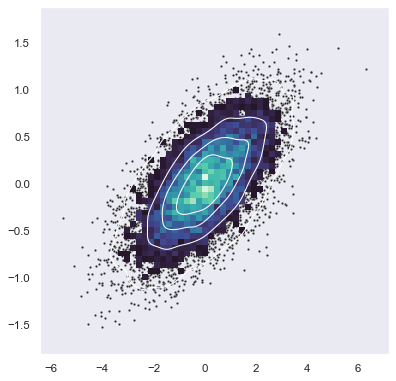
\includegraphics[width=4cm]{layered_bivariate_plot}
      \caption{Data visualization produced by Listing~\ref{list:data-visualization}}
      \label{fig:data-visualization}
    \end{figure}
  \end{frame}

\begin{frame}[<+->]
    \frametitle{IDE vs.\ Text Editor}

    \begin{itemize}
        \item When using programming languages, you will need a program to interact with the language.

              \vfill

        \item There is often a choice between an \textit{integrated development environment} (IDE) and a text editor.

            \vfill

        \item Open source IDEs: RStudio, Spyder, Octave (GUI).

            \vfill

        \item Open source text editors: VSCode (new school), Vi(m) and Emacs (\textit{very} old school).

              \vfill
    \end{itemize}

    \begin{alertblock}{General or specific language support}
        IDEs are tailored to specific languages (such as RStudio).
        Text editors tend to be more multi-purpose.
    \end{alertblock}
\end{frame}
\subsection{Writing}

\begin{frame}[<+->]
    \frametitle{Tools for Writing}
    \begin{itemize}
        \item \LaTeX{}
              \note[item]{
                      Perhaps the most popular open-source tool for creating technical documents out there.
                      Primarily used in mathematics and physics, but there are also packages available for chemistry, biology and more.
                  }

              \vfill

        \item git
              \note[item]{
                      A tool for managing different versions of a document.
                      This is useful for tracking changes in any text-based document.
                  }

                  \vfill

        \item Zotero
            \note[item]{%
              Useful for managing bibliographies.
              You can take your RefWorks bibliography, export it
              to \texttt{.bib} file, and then load your library
              into Zotero for offline access.
            }

            \vfill

        \item harper-ls and LanguageTool
              \note[item]{
                      Tools for checking grammar and spelling in text files.
                  }

              \vfill
    \end{itemize}
\end{frame}

\begin{frame}
    \frametitle{Tools for Drawing}
    \begin{columns}
        \begin{column}{0.5\textwidth}
            \begin{figure}
                \centering
                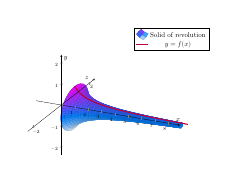
\begin{tikzpicture}[scale=0.25]
                    \begin{axis}[%
                            width=2*175pt,
                            tick label style={font=\scriptsize},
                            colormap/cool,
                            axis on top,
                            axis lines=center,
                            % y dir=reverse,
                            name=myplot, enlargelimits=.1, ymin=-2,
                            ymax=2, xmin=-1, xmax=8, zmin=-2, zmax=2,
                            xtick = {1, 2, ..., 10}, xlabel=$x$,
                            ylabel=$z$, zlabel=$y$]
                        % [view={60}{30}]
                        \addplot3[surf, samples=50, domain=1:9,y
                                domain=0:2*pi, z buffer=sort]
                        % ({(2 + tan(deg(y)))*cos((deg(x)))}, {(2 +
                        % cos(x)) * sin(x)}, {x});
                        (x, {(1/x) * cos(deg(y))}, {(1/x) *
                                sin(deg(y))}); \addlegendentry{Solid of
                        revolution}; \addplot3[samples = 50, samples
                                y = 0, domain = 1:9.5, smooth, ultra thick,
                                purple, z buffer = sort] (x, 0, {1/x});
                        \addlegendentry{$y = f(x)$};
                        % \addplot3[samples = 500, domain = 0:3, y
                        % domain = 0:2*pi, blue!30, opacity = 0.5, z
                        % buffer = sort] (9, {x * cos(deg(y))}, {x *
                        % sin(deg(y))});
                    \end{axis}
                \end{tikzpicture}

                \caption{A PGFPlots drawing}
                \label{fig:pgfplots}
            \end{figure}
        \end{column}
        \begin{column}{0.5\textwidth}
            \begin{itemize}
                \item matplotlib

                      \vfill

                \item pandas

                      \vfill

                \item TikZ/PGFPlots

                      \vfill

                \item Inkscape
            \end{itemize}
        \end{column}
    \end{columns}
\end{frame}

\begin{frame}[<+->]
    \frametitle{Composability Again}
    \begin{itemize}
        \item The tools mentioned so far are not mutually exclusive!

              \vfill

        \item These tools have specific purposes, but can be chained together to form a powerful workflow.

              \vfill

              \begin{exampleblock}{Solving a Math Problem}
                  The expanded form of \( {(x-3)}^5 \) is \( x^{5} - 15 \, x^{4} + 90 \, x^{3} - 270 \, x^{2} + 405 \, x - 243 \).
              \end{exampleblock}

              \vfill
    \end{itemize}
\end{frame}

\subsection{Publicizing}

\begin{frame}[<+->]
    \frametitle{Sharing Your Work}
    Platforms for distributing work:
    \begin{itemize}
        \item \href{https://www.github.com}{GitHub}
              \note[item]{GitHub is owned by Microsoft, but allows some free storage.
                      Beware of AI training!
                  }

              \vfill

        \item personal website.

              \vfill
    \end{itemize}

    \onslide{%
    \begin{alertblock}{Dangers of Sharing Work}
        You should be careful when sharing potentially sensitive work.
        Always check with your advisor and collaborators!
    \end{alertblock}
    }

    \vfill
\end{frame}

\begin{frame}[<+->]
    \frametitle{Literate Programming}
    \begin{itemize}
        \item Work or results that depend on computer analysis can be shared using Jupyter Notebooks.
              \note[item]{%
                      Other tools include Sweave/knitr for R, and Quarto for more general languages.
                  }

              \vfill

        \item Sharing code and a narrative is often more instructive than just sharing the code itself.
              See: \href{https://gwosc.org/tutorials/}{gravity wave notebooks}.
              \note[item]{%
                      Notebooks can also be hosted via Google Colab for interactivity.
                  }

              \vfill
    \end{itemize}
\end{frame}

\begin{frame}
    \frametitle{Licensing Your Work}
    If you are going to share your work, you should specify a license that outlines the following:
    \begin{itemize}
        \item<2-> how your work can be modified and shared.
              \note<2->[item]{%
                      GitHub will actually prompt you to provide a license.
                  }

              \vfill

        \item<3-> in what contexts your work can be used.
              \note<3->[item]{In particular, can it be used in proprietary software?}

              \vfill

    \end{itemize}

    \onslide<4->{%
    \begin{alertblock}{Choosing a License}
        To walk you through the process of choosing a license, you can use tools such as \href{https://choosealicense.com/}{https://choosealicense.com/}.
    \end{alertblock}
    }
\end{frame}

\section{Conclusion}

\begin{frame}[<+->]
    \frametitle{Conclusion}
    \begin{itemize}
        \item Open source tools can form the basis of a powerful workflow.

              \vfill

        \item Despite their utility, these tools often take longer to learn and are not as immediately intuitive as their proprietary counterparts.

              \vfill

        \item You need to decide if they are appropriate for your project!

              \vfill
    \end{itemize}
\end{frame}

\begin{frame}[allowframebreaks]
    \printbibliography%
\end{frame}

\begin{frame}
    % \frametitle{Presentation Repository}
    \begin{center}
        \hypersetup{%
          urlcolor=black,
        }
        \qrcode[height=2in]{https://github.com/j-oldroyd/summer-2026-foss-talk}
    \end{center}
\end{frame}
\end{document}

%%% Local Variables:
%%% TeX-master: t
%%% TeX-engine: luatex
%%% bibtex-dialect: biblatex
%%% End:
